\documentclass{industrial-development}
\graphicspath{{12-knowledge-management/}}

\title{Управление знаниями в процессе промышленной разработки и задачи документирования программного обеспечения}
\author{Смирнов Дмитрий Владиславович, ПИЭ-21 МО}
\date{}

\begin{document}

\begin{frame}
  \titlepage
\end{frame}


\section{Управление знаниями в процессе промышленной разработки}

\subsection{Что это такое?}

\begin{frame} \frametitle{Управление знаниями в промышленной разработке}
  \begin{block}{Что это такое?}
  Управление знаниями (Knowledge Managment) - это процесс создания, накопления, приобретения, распределения и применения знаний на практике. Система знаний содержит ответы на вопросы,  как лучше решать те или иные задачи, опыт и знания сотрудников, список полезной литературы . Построение системы управления знаниями в IT компании — сложная и необходимая задача.
  \end{block}
\end{frame}

\subsection{Что входит в систему знаний?}

\begin{frame} \frametitle{Управление знаниями в промышленной разработке}
  \begin{block}{Что входит в систему знаний?}
  \end{block}
  
  \begin{itemize}
  \item принципы работы компании, её миссия и ценности
  \item материалы, которые обязаны изучить новые сотрудники
  \item подборка полезных ссылок на статьи, книг и других материалов
  \item список частых вопросов и ответы на них
  \item базу обучающих видео, записей вебинаров
  \item описание рабочих процессов компании
  \item лайфхаки и полезные рекомендации для повышения продуктивности
  \item навыки применения различных технологий
  \item личный опыт и знания сотрудников
  \item информация о корпоративных стандартах
  \end{itemize}
\end{frame}

\subsection{Преимущества внедрения базы знаний}

\begin{frame} \frametitle{Управление знаниями в промышленной разработке}
  \begin{block}{Преимущества внедрения базы знаний}
  \end{block}
  
  \begin{itemize}
  \item быстрая адаптация новых сотрудников;
  \item если компанию покидает опытный сотрудник, то его знания остаются в базе
  \item быстрое решение однотипных задач
  \item быстрый поиск ответов на вопросы
  \end{itemize}
\end{frame}

\lecturenotes
Предположим, что в компании появился новый программист. Новичку нужно освоиться, познакомиться со стандартами компании. Чем больше времени на это потребуется, тем больше потерь несёт компания. Если в компании нет базы знаний, адаптация новичка затянется. Ведь ему придётся до многого доходить самостоятельно, он будет делать ошибки при выполнении стандартных задач и постоянно отвлекать коллег вопросами.
Опытные и талантливые сотрудники — это конкурентное преимущество компании. Такие специалисты действуют проактивно, знают лучшее решение для каждой задачи и быстро реагируют на нестандартные ситуации. Секрет их успеха в накопленных знаниях и опыте. Уход опытного сотрудника — большая потеря. Поэтому сохранить знания в компании — стратегическая задача. Её помогает решить менеджмент знаний— работа, направленная на сохранение, распределение и применение знаний в компании. 
Решение однотипных задач. В любой компании есть однотипные задачи, с которыми сотрудники сталкиваются регулярно. Однако без базы знаний каждый сотрудник справляется с ними по-своему, не подозревая, что коллега нашёл лучшее решение. Менеджмент знаний позволяет собрать базу лучших решений для каждой задачи, чтобы все сотрудники работали максимально эффективно. 

\subsection{Инструментальные средства управления знаниями}
\begin{frame} \frametitle{Инструментальные средства управления знаниями}
  \begin{block}{Наиболее популярные средства управления знаниями}
  \end{block}
  
  \begin{itemize}
  \item специальные компьютерные программы
  \item онлайн-сервисы (Evernote, Google Диск)
  \item общие папки на сетевом диске
  \item корпоративные порталы (создание корпоративной энциклопедии Wiki, Howto, рубрики «Вопросы-Ответы»)
  \end{itemize}
\end{frame}

\lecturenotes
 Существует большое количество способов ведения системы знаний. Каждая компания решает для себя удобный способ: это может быть один документ с интерактивным содержанием или система со сложной иерархией.

\subsection{Корпоративные Wiki}
\begin{frame} \frametitle{Корпоративные Wiki}
  \begin{block}{Особеннности данного инструмента}
 Корпоративная вики - программное обеспечение с использованием вики-технологий, предназначенное для использования в корпоративной информационной системе, для обеспечения внутрикорпоративного управления знаниями.
  \end{block}
\end{frame}

\subsection{Возмложности Wiki}
\begin{frame} \frametitle{Корпоративные Wiki}
  \begin{block}{Возможности}
   \end{block}
  
  \begin{itemize}
  \item создание новых страниц, содержащих ссылки на другие корпоративные информационные ресурсы
  \item структурирование информации 
  \item вики позволяет структурировать выражение мнений по конкретному вопросу на одной странице
  \item разграничение прав и ролей
  \item поиск по базе знаний
  \end{itemize}
\end{frame}

\lecturenotes
1. Возможность быстро создавать новые страницы, содержащих ссылки на другие корпоративные информационные ресурсы, ускоряя тем самым формирование базы знаний.
2. Структурирование информации. Вики позволяют пользователям структурировать как новую, так и имеющуюся информацию.
3. Формирование консенсуса. Вики позволяет структурировать выражение мнений по конкретному вопросу на одной странице. Эта функция очень полезна при написании документации, подготовки презентаций, когда мнения участников проекта расходятся.
4. Разграничение прав и ролей. Пользователям может быть отказано в доступе для просмотра и/или редактирования данной страницы, в зависимости от их роли в организации и данном проекте.
5. Возможность поиска по базе знаний.

\subsection{Пример базы знаний в IT}
\begin{frame} \frametitle{Пример базы знаний в IT}
\centerline{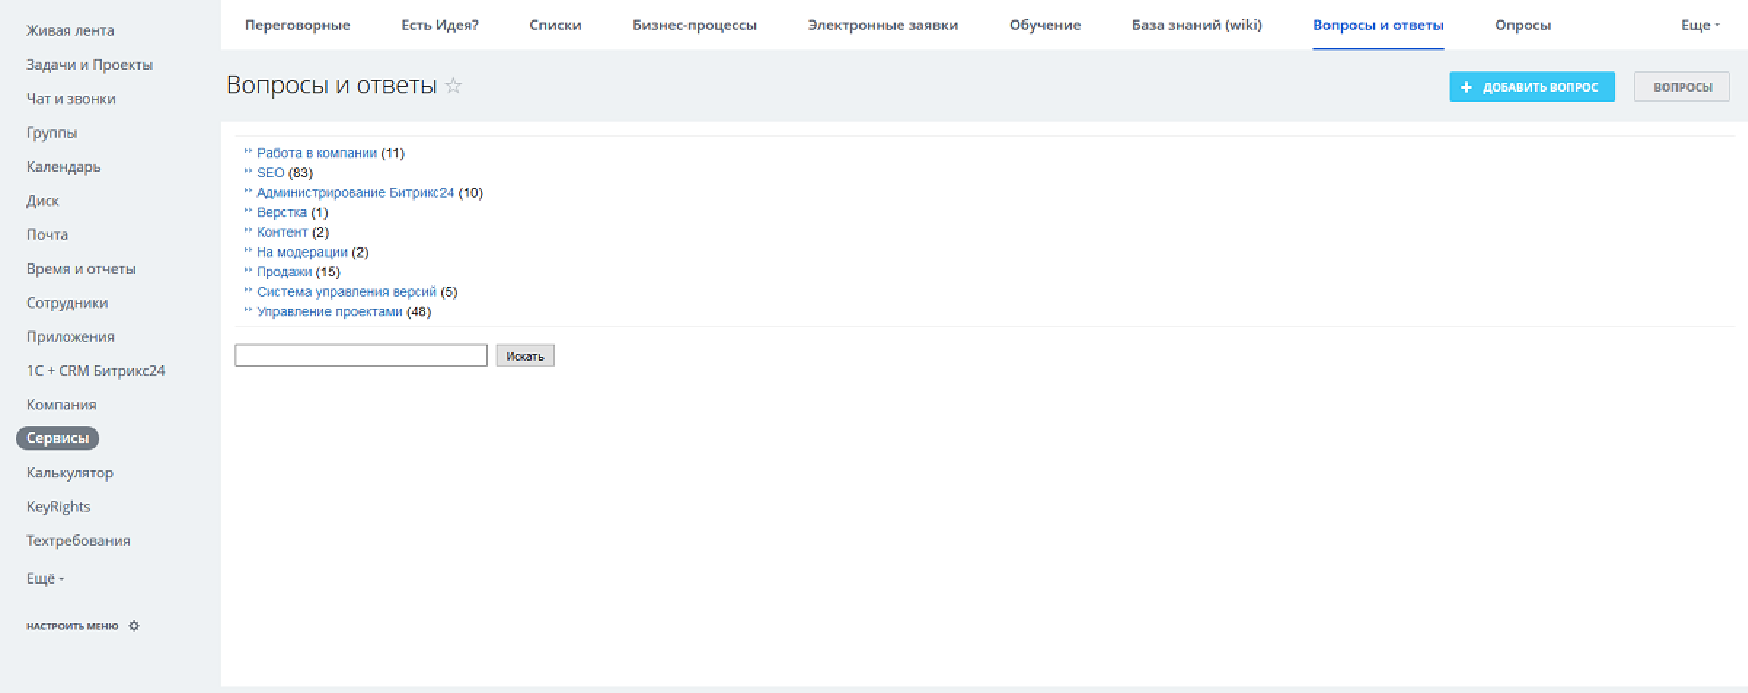
\includegraphics[width=1\textwidth]{voprosy-otvety.pdf}}
\centerline{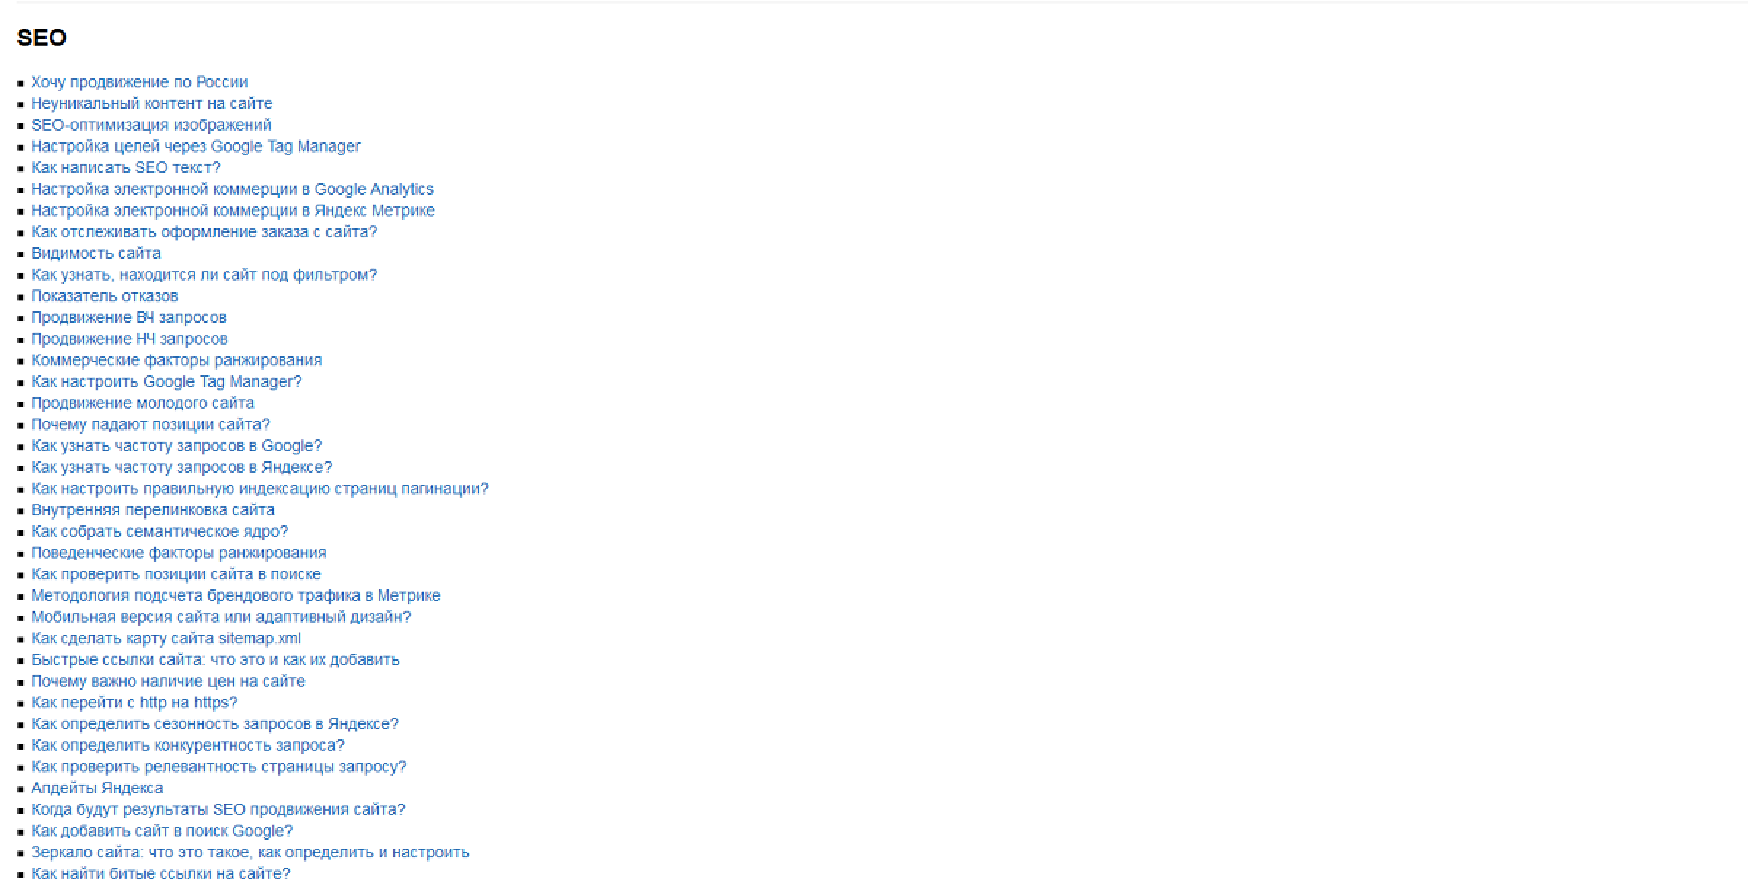
\includegraphics[width=1\textwidth]{seo.pdf}}
\end{frame}

\section{Документация ПО}
\subsection{Зачем она нужна?}
\begin{frame} \frametitle{Документация ПО}
  \begin{block}{Зачем она нужна?}
\dots
  \end{block}
  
  \begin{itemize}
  \item Чтобы быстро понять логику кода
  \item Чтобы легко поддерживать код другим программистами
  \item Чтобы пользователям было легче использовать программу
  \end{itemize}
\end{frame}

\subsection{Типы документации ПО}
\begin{frame} \frametitle{Документация ПО}
  \begin{block}{Типы документации ПО}
Существует три основных типа документации на ПО: 
  \end{block}
  \begin{itemize}
  \item архитектурная/проектная — обзор программного обеспечения, включающий описание рабочей среды и принципов, которые должны быть использованы при создании ПО
  \item пользовательская — руководства для конечных пользователей, администраторов системы и другого персонала
  \item техническая — документация на код, алгоритмы, интерфейсы, API
  \end{itemize}
\end{frame}

\subsection{Архитектурная/проектная документация}
\begin{frame} \frametitle{Документация ПО}
  \begin{block}{Архитектурная/проектная документация}
 Проектная документация обычно описывает продукт в общих чертах. Описываются причины, почему какой-либо класс сконструирован определённым образом, выделяются паттерны, в некоторых случаях даже даются идеи как можно будет выполнить улучшения в дальнейшем. Ничего из этого не входит в техническую или пользовательскую документацию, но всё это действительно важно для проекта.
  \end{block}
\end{frame}

\subsection{Пользовательская документация}
\begin{frame} \frametitle{Документация ПО}
  \begin{block}{Пользовательская документация}
Пользовательская документация представляет собой руководство пользователя, которое описывает как можно пользоваться программой.
  \end{block}
\end{frame}

\lecturenotes
Пользовательская документация описывает то, как использовать программу.
Обычно, пользовательская документация представляет собой руководство пользователя, которое описывает каждую функцию программы, а также шаги, которые нужно выполнить для использования этой функции. Хорошая пользовательская документация предоставляет инструкции о том, что делать в случае возникновения проблем. Руководство должно иметь чёткую структуру; очень полезно, если имеется сквозной предметный указатель. Логическая связность и простота также имеют большое значение.
Существует три подхода к организации пользовательской документации. Вводное руководство, наиболее полезное для новых пользователей, последовательно проводит по ряду шагов, служащих для выполнения каких-либо типичных задач. Тематический подход, при котором каждая глава руководства посвящена какой-то отдельной теме, больше подходит для совершенствующихся пользователей. В последнем, третьем подходе, команды или задачи организованы в виде алфавитного справочника — часто это хорошо воспринимается продвинутыми пользователями, хорошо знающими, что они ищут. Жалобы пользователей обычно относятся к тому, что документация охватывает только один из этих подходов, и поэтому хорошо подходит лишь для одного класса пользователей.
Во многих случаях разработчики программного продукта ограничивают набор пользовательской документации лишь встроенной системой помощи, содержащей справочную информацию о командах или пунктах меню. Работа по обучению новых пользователей и поддержке совершенствующихся пользователей перекладывается на частных издателей, часто оказывающих значительную помощь разработчикам. 

\subsection{Техническая документация}
\begin{frame} \frametitle{Документация ПО}
  \begin{block}{Техническая документация}
Техническая документация кода - это вставка в код определенных комментариев, которые позволяют в дальнейшем упростить работу с кодом, как автору, так и другим программистам. Многие программисты не любят это дело и пытаются всячески избежать этой работы всеми доступными способами. Отсутсвие документации кода приводит к плохой его читаемости и к сложному техническому обслуживанию для других членов команды.
  \end{block}
\end{frame}

\lecturenotes
Техническое документирование кода является трудоемким процессом.  Для того, чтобы обеспечить более быстрый процесс подготовки документации необходимо использовать автоматизированные системы.
На практике же далеко не каждый программный проект может похвастаться, что у него имеется полная и актуальная в любой момент времени документация на разрабатываемый программный код.
Основной причиной этого является то, что разработка полной и актуальной документации является весьма трудоемким мероприятием и занимает сопоставимое (если не больше) время по сравнению с разработкой самого программного кода время.

\subsection{Генераторы документации}
\begin{frame} \frametitle{Документация ПО}
  \begin{block}{Генераторы документации}
  \end{block}
Генератор документации -  программа, позволяющая получать документацию, предназначенную для программистов и для конечных пользователей системы, по особым образом комментированному исходному коду и, в некоторых случаях, по исполняемым модулям (полученным на выходе компилятора).Обычно генератор анализирует исходный код программы, выделяя синтаксические конструкции, соответствующие значимым объектам программы (типам, классам и их членам/свойствам/методам, процедурам/функциям и т. п.).  На основе всей собранной информации формируется готовая документация, как правило, в одном из общепринятых форматов — HTML, HTMLHelp, PDF, RTF и других. 
\end{frame}
\lecturenotes

\subsection{Преимущества автогенерации документации}
\begin{frame} \frametitle{Документация кода}
  \begin{block}{Преимущества автогенерации документации}
  \end{block}
  \begin{itemize}
  \item Документация становится в большей степени согласованной с программным кодом, то есть более точной и актуальной
  \item Экономится значительное количество времени и усилий, требуемых для разработки документации. Освобождаемые время и ресурсы можно применить для улучшения качества документации
  \item Более простым становится процесс изменения формата или стиля подачи документации. При наличии собственного генератора не надо менять формат каждого документа, достаточно изменить шаблон
  \item Документация формируется значительно быстрее
  \end{itemize}
\end{frame}
\lecturenotes

\begin{frame} \frametitle{Документация кода}
  \begin{block}{Программы для автоматической генерации документации}
 Для автоматической генерации документации кода используются специальные программы. Например:
  \end{block}
  \begin{itemize}
  \item DOXYGEN
  \item SPHINX
  \item DR. EXPLAIN
  \item PHPDOCUMENTOR
  \end{itemize}
\end{frame}
\lecturenotes
Наиболее популярные программы для генерации документации:
Doxygen является отличным инструментом для генерации документации из исходного кода. Инструмент нацелен на документирование программного обеспечения, написанного на языке C++, однако на самом деле данная система поддерживает гораздо большое число других языков, таких как: C, Objective-C, C#, PHP, Java, Python, IDL, Fortran, VHDL, Tcl, и частично D. С помощью Doxygen, вы можете создать онлайн HTML документацию. Doxygen — консольная программа в духе классической Unix. Она работает подобно компилятору, анализируя исходные тексты и создавая документацию. Самым большим преимуществом использования Doxygen является то, что вы будете иметь последовательность всей документации исходного кода. Она также может помочь вам создавать структуру кода с использованием недокументированных исходных файлов.
Sphinx это популярный инструмент позволяющий создавать текстовые документы и преобразовывать их в различные форматы. Это удобно при использовании систем управления версиями, предназначенных для отслеживания изменений. Он доступен по лицензии BSD и поддерживает несколько языков программирования, таких как Python, C и C++. Он может быть использован как для проектной документации так и для документации кода. Sphinx избавляет от рутинных действий и предлагает автоматическую функциональность для решения типовых проблем, например, индексирования заголовков и специального выделения кода (например, при включении в документ фрагментов кода) с соответствующим выделением синтаксиса.
Frontend разработка также, в определенной степени, требует документирования. Создавать документацию как для обычных, так и онлайн-приложений, написанных на любом языке программирования, в любой среде разработки, с применением любого фреймворка поможет DR. EXPLAIN. Он фильтрует ключевые элементы интерфейса, а затем извлекает связанные с ним мета данные. После этого, вы можете изменить полученную информацию, чтобы быстро создать документацию интерфейса.  
Если вы PHP разработчик и хотите сгенерировать документацию кода из исходного кода, стоит рассмотреть PhpDocumentor. В основе работы системы лежит парсинг логической структуры PHP кода (классы, функции, переменные, константы) и привязка к ней комментариев, написанных по определенным стандартам. Инструмент также может помочь вам генерировать отчеты и графики и повысить общее качество кода.

\begin{thebibliography}{99}
\end{thebibliography}

\end{document}
